\chapter{绪论}

无论使用texstudio还是vscode,建议
\begin{itemize}
	\item 分章节写,input进来,可以只编译当前章节,其他注释掉,节约编译时间,不然当工程比较大时,统一编译很慢
	\item 不同图片、表格也写在单独tex中,input进来
\end{itemize}

input进来的好处是看起来清爽,而且注释方便

\section{研究背景及意义}


\begin{table}[h]  
		\centering  
		\fontsize{10}{10}\selectfont  
		\caption{\rm 在Rain12\upcite{gmm}、Rain1200\upcite{didmdn}和Test1000\upcite{spanet}数据集上的定量结果(PSNR$\uparrow$与SSIM$\uparrow$)比较,$\uparrow$表示该评价指标数值越大算法性能越好,最佳与次佳结果分别用黑体和下划线标出。*表示本文所提方法。} 
		\label{tab:rain12-rain1200-test1000}
		\begin{threeparttable}  
			\begin{tabular}{c|cc|cc|cc}
				\toprule  
				\multirow{2}{*}{\makecell{Methods\\[-.15cm]}}& 
				\multicolumn{2}{c|}{Rain12}&\multicolumn{2}{c|}{Rain1200}&\multicolumn{2}{c}{Test1000}\cr  
				\cmidrule(lr){2-3} \cmidrule(lr){4-5}\cmidrule(lr){6-7}   
				&PSNR$\uparrow$ &SSIM$\uparrow$&PSNR$\uparrow$&SSIM$\uparrow$&PSNR$\uparrow$&SSIM$\uparrow$\cr  
				\midrule 
				 
				DSC\upcite{dsc}  &29.98&0.8654  &21.44&0.7896&32.33&0.9335\cr  
				GMM\upcite{gmm} &32.15&0.9145&22.75&0.8352&32.99&0.9475\cr 
				CNN~\upcite{cnn}   &33.33&0.9199&23.55&0.8352&31.31&0.9304\cr
				JORDER~\upcite{jorder}   & {36.15}&0.9548&25.71&0.8074&35.72&{0.9776}\cr
				DDN~\upcite{ddn}   & 29.84&0.9049& 30.08&0.8791&34.88&0.9727\cr 
				DID-MDN~\upcite{didmdn} &29.49&0.9031&29.65&0.9016&28.96&0.9457\cr
				%SEMI\upcite{semi} &- &-&26.05&0.8220&-&-\cr
				PreNet~\upcite{prenet} & \underline{36.66}&0.9610&30.56&0.8750&30.31&0.9538\cr
				SPANet~\upcite{spanet} &32.71 &0.9285&30.05&\bf 0.9342&38.53& \underline{0.9875}\cr
				\midrule
				CODE-Net* &{ 36.21}&\underline{ 0.9618}&{ \underline {33.31} }&0.9174&\underline{ 38.88}&0.9867\cr
				mCODE-Net*  &\bf { 36.79}&{ \bf {0.9639}}&{\bf {34.03}}&\underline{ 0.9281}&{\bf 39.85}&\bf 0.9879\cr  				
				\bottomrule  
			\end{tabular} 
		\end{threeparttable}  
\end{table}  

\begin{figure}[t] 
	\centering
	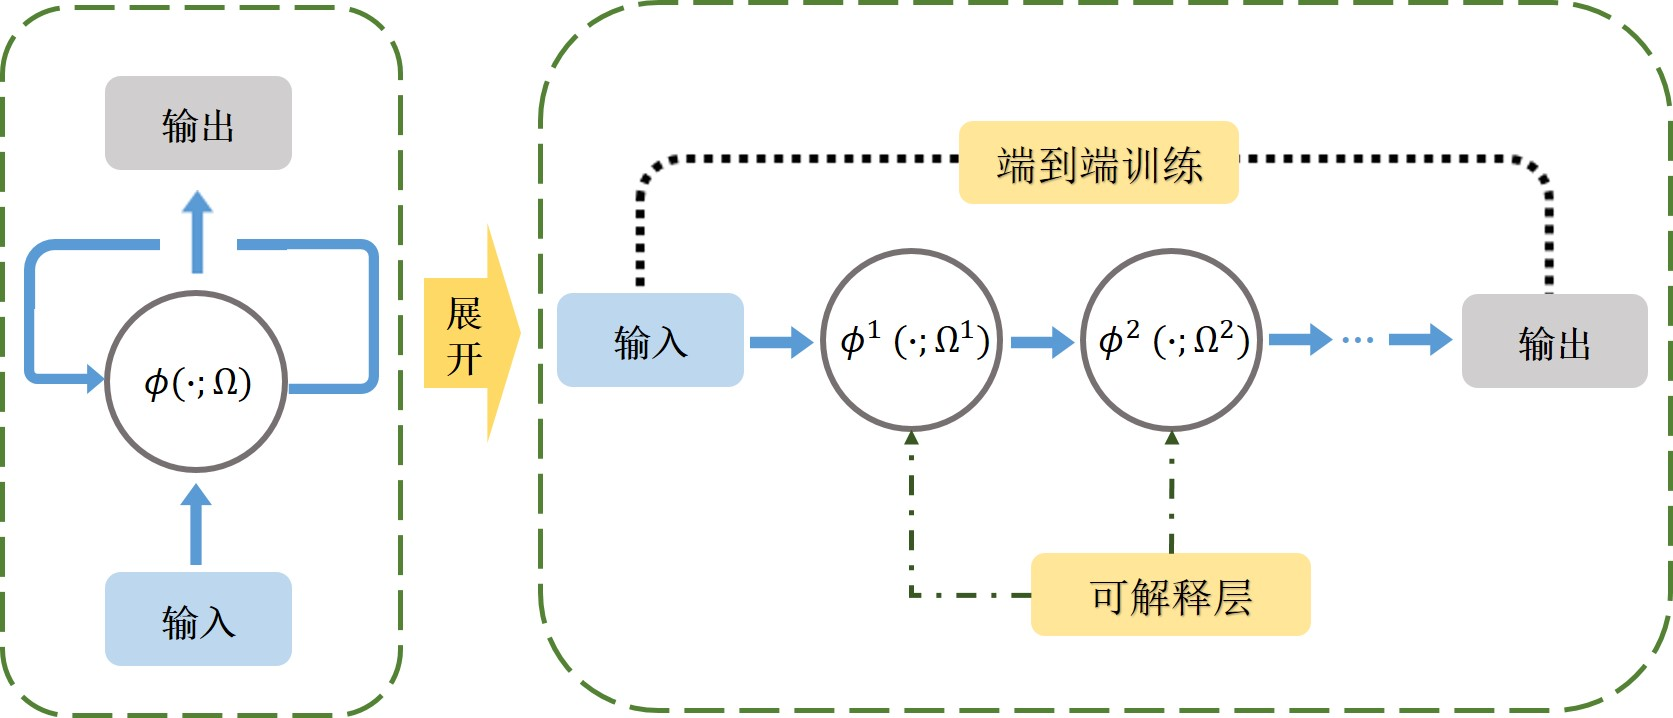
\includegraphics[width=0.99\linewidth]{figures/unroll.jpg}
	\caption{ \rm Deep Unfolding技术示意图。}
	\label{fig:unrolling}	
\end{figure}